\documentclass[11pt]{article}
\usepackage{amsmath, amssymb, amscd, amsthm, amsfonts}
\usepackage{graphicx}
\usepackage{hyperref}
\usepackage{biblatex}
\usepackage{subfig}


\addbibresource{references.bib}

\oddsidemargin 0pt
\evensidemargin 0pt
\marginparwidth 40pt
\marginparsep 10pt
\topmargin -20pt
\headsep 10pt
\textheight 8.7in
\textwidth 6.65in
\linespread{1.2}


\title{Numerical Methods for Solving Fermion System Ground State}
\author{Zhongwei Wang}
\date{2022 Autumn}

\newtheorem{theorem}{Theorem}
\newtheorem{lemma}[theorem]{Lemma}
\newtheorem{conjecture}[theorem]{Conjecture}

\newcommand{\rr}{\mathbb{R}}

\newcommand{\al}{\alpha}
\DeclareMathOperator{\conv}{conv}
\DeclareMathOperator{\aff}{aff}

\begin{document}

\maketitle

\begin{abstract}\footnote[1]{Source code available on \href{https://github.com/Wang-Zhongwei/Many-body-ground-state-energy-by-VMC-and-SCF/tree/main}{Github}}
This article presents numerical methods for solving the ground state of the Fermion system, including self-consistent field (SCF) theory and Variational Monte Carlo (VMC). 
As a demonstration of the algorithms, Helium and Beryllium atoms are solved independently by each algorithm in succession. 
It shows that each method produces result within 1\% of the exact value. After considering the correlation term in VMC the error was further reduced to less than 0.01\%. However SCF does not include electron correlation while VMC is relatively slow. Future work could look into combining the two methods to achieve both high efficieny and accuracy. 

\end{abstract}

\section{Introduction}\label{section-introduction}
Hamiltonians for a Fermion system has a general expression as follows:
\begin{equation}\label{eq:hamiltonian}
\hat{H} = \frac{1}{2}\sum_{i}\nabla_i^2  - \sum_i \frac{Z}{r_i} + \frac{1}{2}\sum_{i \neq j} \frac{1}{|r_i-r_j|},
\end{equation}
\begin{itemize}
    \item first two terms are called single-body terms, representing electron-nucleus interaction;
    \item last term called many-body term, representing electron-electron interaction, which can be then broken down into 
    direct term $J$ and exchange term $K$; 
\end{itemize}
Without the last term, system eigen states would be simply produced by Slater determinants. Otherwise, the system is not solvable analytically.

Common numerical methods for solving many-body quantum systems include Variational Monte Carlo (VMC) \cite{First_VMC} methods, density functional theory (DFT) \cite{First-DFT}, and Self-consistent field (SCF) \cite{Early-SCF} theory. 
These methods use various computational techniques to approximate the solutions to many-body quantum systems. This article, in particular, uses self-consistent field (SCF) theory and Variational Monte Carlo (VMC) to solve the ground state of Helium and Beryllium. 
There are several mature libraries and software packages for quantum Monte Carlo and density functional theory simulation. For example, \href{https://www.quantum-espresso.org/}{Quantum ESPRESSO}, \href{https://qmcpack.org/}{QMCPACK}, \href{https://vallico.net/casinoqmc/}{CASINO} for VMC; \href{https://www.nwchem-sw.org/}{NWChem} and \href{https://dftbplus.org/}{DFTB+} for DFT. 

But for the purpose of illumination only, in this article, I opt to implement them ground up. For the next two chapters, I am going to review the principles of the two algorithms and lay out the procedure to solve the specific problems in concern, which is the ground state of Helium and Beryllium.

\section{Principle}
In this chapter, the derivation of the whole theory is not the main focus. One can refer to \cite{Derivation_of_Fock_matrix} \cite{Review_of_VMC} for detailed derivations. Instead, we review important conclusions about and stipulate notations for SCF and VMC.
\subsection{Hartree-Fock equations}
The Hartree-Fock self-consistent field (SCF) theory is a method used in quantum chemistry to approximate the wave function and energy of a many-electron system. 
The theory is based on the Hartree-Fock approximation, which assumes that the many-electron wave function can be represented as a determinant, known as the Slater determinant, of single-electron wave functions (often not orthogonal), or orbitals. 
The SCF method involves iteratively solving the Hartree-Fock equations to determine the orbitals and the energy of the system and then using these solutions as the starting point for the next iteration. 
This process is repeated until the solutions converge to a self-consistent set of orbitals and energy, which represents the best approximation of the true wave function and energy of the system.

Closed and open-shell systems are usually treated differently. In a closed shell system, every electron got paired with another with the same spatial orbit but opposite spin so the number of basis functions is equal to one-half of the total number of electrons. The SCF procedure typically converges quickly and accurately, since the electrons are paired and the total spin is zero. In an open shell system, on the other hand, the SCF procedure may take longer to converge and may not be as accurate, due to the presence of unpaired electrons and non-zero total spin. \cite{closed-vs-open-shell} Considering the examples used in this article are inert gases, it makes more sense to use closed-shell SCF.


Adapted from original Hamiltonian \ref{eq:hamiltonian}(How?). The Hartree-Fock equation for a closed-shell atomic system reads as follows:
\cite{Fock_matrix_source}
\begin{equation}
\label{eq:hartree-fock}
\hat{f}(r_i) = \hat{h}(r_i)+\sum_{a=1}^{N/2}(2\hat{J}_a(r_i)-\hat{K}_a(r_i))
\end{equation}
where
\begin{itemize}
    \item $\hat{f}(r_i)$: Fock operator;
    \item $\hat{h}(r_i)$: single body operator;
    \item $\hat{J}_a(r_i)$: direct operator attributed to electron-electron coulomb repulsion;
    \item $\hat{K}_a(r_i)$: exchange operator attributed to same-spin electron exchange effect. The factor is half of that of the direct operator. 
\end{itemize}
One strong assumption of SCF is that the composite wavefunction can be written as the determinant of basis functions evaluated at each electron position. 

\begin{align*}
    \Psi(r_1, r_2, ..., r_N) &= 
    \begin{vmatrix}
    \psi_1(r_1) & \psi_2(r_1)  & \cdots & \psi_N(r_1) \\ 
    \psi_1(r_2) & \psi_2(r_2) & \cdots & \psi_N(r_2) \\ 
    \vdots & \vdots& \ddots & \vdots \\
    \psi_1(r_N) & \psi_2(r_N) & \cdots & \psi_N(r_N) \\ 
    \end{vmatrix} \\
\end{align*}

Remeber set of basis $\{\psi_1, ... , \psi_N\}$ is not neccessarily orthogonal. The Fock operator under the representation becomes:
\begin{equation}\label{eq:fock-representation}
    F_{\mu\nu}=H^{core}_{\mu\nu} + G_{\mu\nu}
\end{equation}
where 
\begin{itemize}
    \item $H^{core}_{\mu \nu} = \int{dv_1 \phi_{\mu}^*(r_1)\hat{h}_1(r_1)\phi_{\nu}(r_1)}$; $\hat{h}_1(r_1)=-\frac{1}{2}\nabla^2_1-\frac{Z}{r_1}$; single body term.
    \item $G_{\mu\nu} = \sum_{a=1}^{N/2}(2(\mu\nu|aa)-(\mu a|a\nu))$
    \item $(\mu\nu|aa)=\int{dv_1 dv_2 \psi_{\mu}^*(r_1)\psi_{\nu}(r_1) \frac{1}{r_{12}} \psi_a^*(r_2)\psi_a(r_2)}$; direct term.
    \item $(\mu a|a\nu)=\int{dv_1 dv_2 \psi_{\mu}^*(r_1)\psi_{a}(r_1) \frac{1}{r_{12}} \psi_a^*(r_2)\psi_{\nu}(r_2)}$; exchange term.
\end{itemize}

The relation between energy and the Fock operator is:
\begin{equation}
    E(\Psi(r_1, r_2, ..., r_N)) = \sum_{\mu, \nu} (H_{\mu\nu} + \frac{1}{2}G_{\mu\nu}) = \frac{1}{2} \sum_{\mu, \nu} (H_{\mu\nu}^{core} + F_{\mu\nu})
\end{equation}

However, it is more convenient to choose another set of basis $\{\phi_1, \phi_2, ... \phi_N\}$ with relation $\psi_j = \sum_{i}\phi_{i} \cdot C_{ij}$, where $C_{ij}$ is called the coefficient matrix. After the transformation fock matrix of the system becomes:

\begin{flalign*}
    F_{\mu\nu} & = H_{\mu\nu} + \sum_{a}^{N/2}\sum_{\lambda, \sigma}C_{\lambda a}C_{\sigma a} (2(\mu\nu|\lambda\sigma) - (\mu\sigma|\lambda\nu)) \\ 
    & = H_{\mu\nu} + \sum_{\lambda, \sigma} P_{\lambda\sigma}((\mu\nu|\lambda\sigma) - \frac{1}{2}(\mu\sigma|\lambda\nu))
\end{flalign*}
where 
\begin{subequations}
    \begin{align}
        P_{\lambda\sigma} &= 2\sum_{a}^{N/2}C_{\lambda a}C_{\sigma a} 
    \end{align}
\end{subequations}
is called density matrix.

The advantage of this approach is that we can calculate and tabulate the matrix elements such as $(\mu\nu|\lambda\sigma)$ once and for all, which is very expensive to calculate. The disadvantage is that the basis set is not orthogonal, which makes the calculation of the energy more complicated. 

By minimizing the energy functional $<\Psi|\hat{H}|\Psi>$ coefficients can be produced by solving eigen equations over and over again. Each time plug in the old coefficients from the last loop and solve the eigen equations again. This is called SCF procedure. The eigen equation to be solved is called Roothaan-Hall Equations \cite{Roothan-Hall}: 

\begin{equation}\label{eq:roothaan-hall}
    FC = S C \epsilon
\end{equation}

where S is the overlap matrix. $S_{ij} := \int{dv\phi^*_i(r)\phi_j(r)}$ The eigenvalues $\epsilon$ are the energies of the basis functions. The eigenvectors $C_{\mu i}$ are the coefficients of the basis functions. I will talk about the precise procedure of implementing solving the Roothan-Hall equation by recursion in chapter \ref{s:scf-procedure}. 
\subsection{Variational Monte Carlo}


\section{Procedure}
\subsection{Model}

For simplicity's sake, the system we only consider is a closed shell system where there are $N/2$ different spatial orbits given $N$ electrons. We assume the form of the atomic wavefunction is 

\begin{equation}
\label{eq:atomic-wavefunction}
    \Psi = Det(\phi_1(r_1), \phi_2(r_2), ..., \phi_N(r_N)) \cdot \prod_{i<j}\exp(\frac{r_{ij}}{2(1 + \beta_{ij}r_{ij})})
\end{equation}
where the determinant part encapsulates the electron exchange effect while the second part includes electron correlation which is not taken care of by the Hartree-Fock approximation. 

Slater-type orbitals are used for basis functions: \cite{hjorthcomputational}
\begin{itemize}
    \item $\phi_{1s}(r_i) = N_{1s}\exp(-\alpha_1 r_i)$
    \item $\phi_{2s}(r_i) = N_{2s}(1 - \alpha_2 r_i / 2)\exp(-\alpha_2 r_i / 2)$
    \item $\mathbf{\phi}_{2p}(r_i) = N_{2p} \alpha_3 \textbf{r} \exp(-\alpha_3 r_i/2)$
    \item $\vdots$
\end{itemize}
where $\alpha$ and $\beta$ reflect shielding and correlation effect physically. Those parameters are optimized by minimizing the energy of the system. Since SCF is usually faster than VMC, which will be proved in later implementations. All $\alpha$ will be optimized by SCF by finding the minimum of the convergent energy before all $\beta$ are optimized by VMC by using the very combination of $\alpha$.


\subsection{SCF}\label{s:scf-procedure}
Let's observe the roothaan-hall equation \ref{eq:roothaan-hall} again. $S$ is Hermitian ant thus can be Diagonalized using $S=T^{\dag} \Lambda T$ where $T$ is othornormal. Define another Hermitian matrix $ \chi = T^{\dag}\Lambda^{-1/2} T$ and . One can find that $\chi^{\dag}\chi = \chi^2 = S^{-1}$. Let define $F' = \chi^{\dag} F \chi$ and $C'=X^{-1}C$. Insert $\chi^{-1}\chi$ between $F$ and $C$, $S$ and $C$. We can have the eigen equation as follows:
\begin{equation}
    F' C' = C' \epsilon
\end{equation} 
However, it is not a trivial eigen system problem because $F'$ is implicitly dependent on its eigen vectors $C'$. To solve this, we need to first assume a plausible assumption about $C$ matrix use it as first guess to solve the eigen equation. Then we can use the eigen vectors $C'$ to calculate the new $F'$ and use it to solve the eigen equation again. This process is called recursion. The recursion is terminated when the difference between the new $F'$ and the old $F'$ is small enough. Summarizing the procedure of SCF:
\begin{enumerate}
    \item Specify system and basis set $\{\phi_1, ...,\phi_{N/2}\}$
    \item Calculate one and two-electron integrals
    \item Diagonalise the overlap matrix, to obtain a transformation matrix, $\chi = S^{-1/2}$
    \item Provide an initial guess as to the density matrix. 
    \item Calculate $G$ matrix ($2J-K$)  using $P$ and the two-electron integrals
    \item Obtain Fock matrix from the sum of the core Hamiltonian matrix and  $G$ matrix, $F=H^{core} + G$
    \item Calculate transformed Fock matrix $F'=\chi^{\dag} F \chi$
    \item Diagonalize $F'$ to get $C'$
    \item Calculate the real coefficient matrix $C=\chi C^{'}$
    \item These coefficients form the new matrix $P$
    \item Determine convergence of the density matrix, by comparing the new density matrix with the old density matrix within a specified criterion. If the convergence has not been met then return to step (5) with the new density matrix $P$ to form a new Fock matrix and repeat
    \item If convergence has been met then end the SCF cycle and return desired quantities, e.g. Energy, coefficient matrix.
\end{enumerate}

If convergence has been met then end the SCF cycle and return desired quantities, e.g. Energy, coefficient matrix. The process can be summarized as the following figure:


Now we think SCF as a black box. It takes into parameters like $\alpha$ and $\beta$ of the basis functions and produces energy and a convergent coefficient matrix. The next goal is to find the optimal parameters that make energy as low as possible. This would mean we need to search over the parameter space to find the best configuration of $\alpha$ and $\beta$. Brute force iteration can always achieve the goal, namely, iterate all possible combinations of $\alpha$ and $\beta$ and record the lowest energy. Also, we can vectorize and parallelize the code since the results are independent for a different set of parameters. However, as the number of parameters grows, time complexity grows exponentially. In that case, we have to resort to simulated annealing to probe the optimal parameters. \cite{simulated-annealing}

The process of simulated annealing involves iteratively perturbing the current state of a system and then accepting or rejecting the new state based on its energy. If the new state has a lower energy, it is always accepted. If the new state has a higher energy, it is sometimes accepted, with the probability of acceptance determined by a "temperature" parameter. This temperature is gradually reduced over time, which helps the algorithm escape local minima and converge on the global minimum. Diagrammatically, the process looks like figure \ref{fig:scf flowchart}

\begin{figure}
    \centering
    \subfloat[\centering SCF Procedure]{{\includegraphics[width=5cm]{figs/scf-procedure.png} }}%
    \qquad
    \subfloat[\centering Simulated Annealing Procedure\cite{simulated-annealing-flowchart}]{{\includegraphics[width=5cm]{figs/A-flowchart-of-the-simulated-annealing-algorithm.jpg} }}%
    \caption{Flowchart of SCF algorithms}%
    \label{fig:scf flowchart}%
\end{figure}

\subsection{VMC}
The process of VMC involves two main steps: 
\begin{enumerate}
    \item Finding a trial wave function that is a good approximation of the true ground state wave function
    \item Using Monte Carlo sampling to compute expectation values of the Hamiltonian with respect to the trial wave function.
\end{enumerate}

In the first step, the trial wave function is parameterized using a set of adjustable parameters. These parameters are chosen to minimize the so-called "variational energy", which is the expectation value of the Hamiltonian with respect to the trial wave function. This step is usually performed using some form of optimization algorithm, such as gradient descent or simulated annealing.

In the second step, the trial wave function is used to generate a set of random samples from the many-body system. These samples are then used to compute the expectation values of the Hamiltonian and other physical observables. Because the trial wave function is a good approximation of the true ground state wave function, the expectation values computed using VMC are also good approximations of the true values. As is shown by figure \ref{fig:vmc flowchart}.

\begin{figure}
    \centering
    \includegraphics[width=6cm]{figs/vmc-flowchart.png}
    \caption{Flowchart of VMC algorithms}
    \label{fig:vmc flowchart}%
\end{figure}

\section{Initialization and Setup}

\subsection{SCF}
Prior to implementing SCF, we need to know all the matrix elements involved in equation \ref{eq:fock-representation}. Two electron integrals such as $T_{ij}$ and $V_{ij}$ as well as four electron integrals are first analytically evaluated by Mathematica file $src/main/MatrixElements.nb$. Solved expressions are then imported to python script $src/main/int.py$ so that given each $\alpha$ set, concrete values of matrix elements can be calculated and stored in directory $src/resources/hf$. 

During the simulated annealing process, temperature function is chosen to be decreasing over loop number so that energy could converge to the minimum just like a real annealing process. Refer to the penalty factor (reciprocal of temperature) in $src/main/scf.py$. 

Step length parameter is initially set to .5 and also decreases exponentially over time in order to get better accuracy. In this way, we can keep the local acceptance rate around 25\% all the time which is believed \cite{optimal-mc-acc-rate} to be the best acceptance rate for markov chain monte carlo considering both sampling efficiency and result accuracy.

\subsection{VMC}
Unlike SCF, VMC simulation has two sets of parameters $\alpha$ which is only included in SCF and $\beta$ which captures electron correlation. For the loop that evaluates the averaged local energy, position step length is chosen to be 1.0 Bohr radius in order to reduce covariance. Then we need to find out the optimal set of parameters that produce the lowest energy. There are two methods that try out every possible combination of $\alpha$ and $\beta$. 

For a system with a small number of electrons, it is possible to iterate over the entire parameter space. For helium, $\alpha$ is chosen to be in the range of $[1, 2]$ and $\beta$ is chosen to be in the range of $[0.5, 1.5]$. For beryllium, $\alpha$ is chosen to be in the range of $[1.0, 2.0]$ and $\beta$ is chosen to be in the range of $[1.0, 1.9]$.

\section{Results}
\subsection{SCF}
\subsubsection*{Helium}
Helium has 2 electrons which means we only need $\frac{2}{2}=1$ STO type function as basis. It shows that when $\alpha=1.69$, the converged energy produced by SCF is minimized to be -2.8477 (Hartree). 

Compared with analytical variational method \cite{analytical_variatonal_He}. $\alpha=\frac{27}{16} = 1.6875$ and $E=-2.848$. Numerical result is very close to analytical result. 

\subsubsection*{Beryllium}
For Beryllium two STO basis are needed. After 200 loops of simulated annealing, we can see that minimized energy is $-14.698$, corresponding parameters are $\alpha_{1s}=3.68$ and $\alpha_{2s}=2.13$. Annealing energy and parameter trajectory are shown in figure \ref{fig:be-scf-annealing}.
\begin{figure}
    \centering
    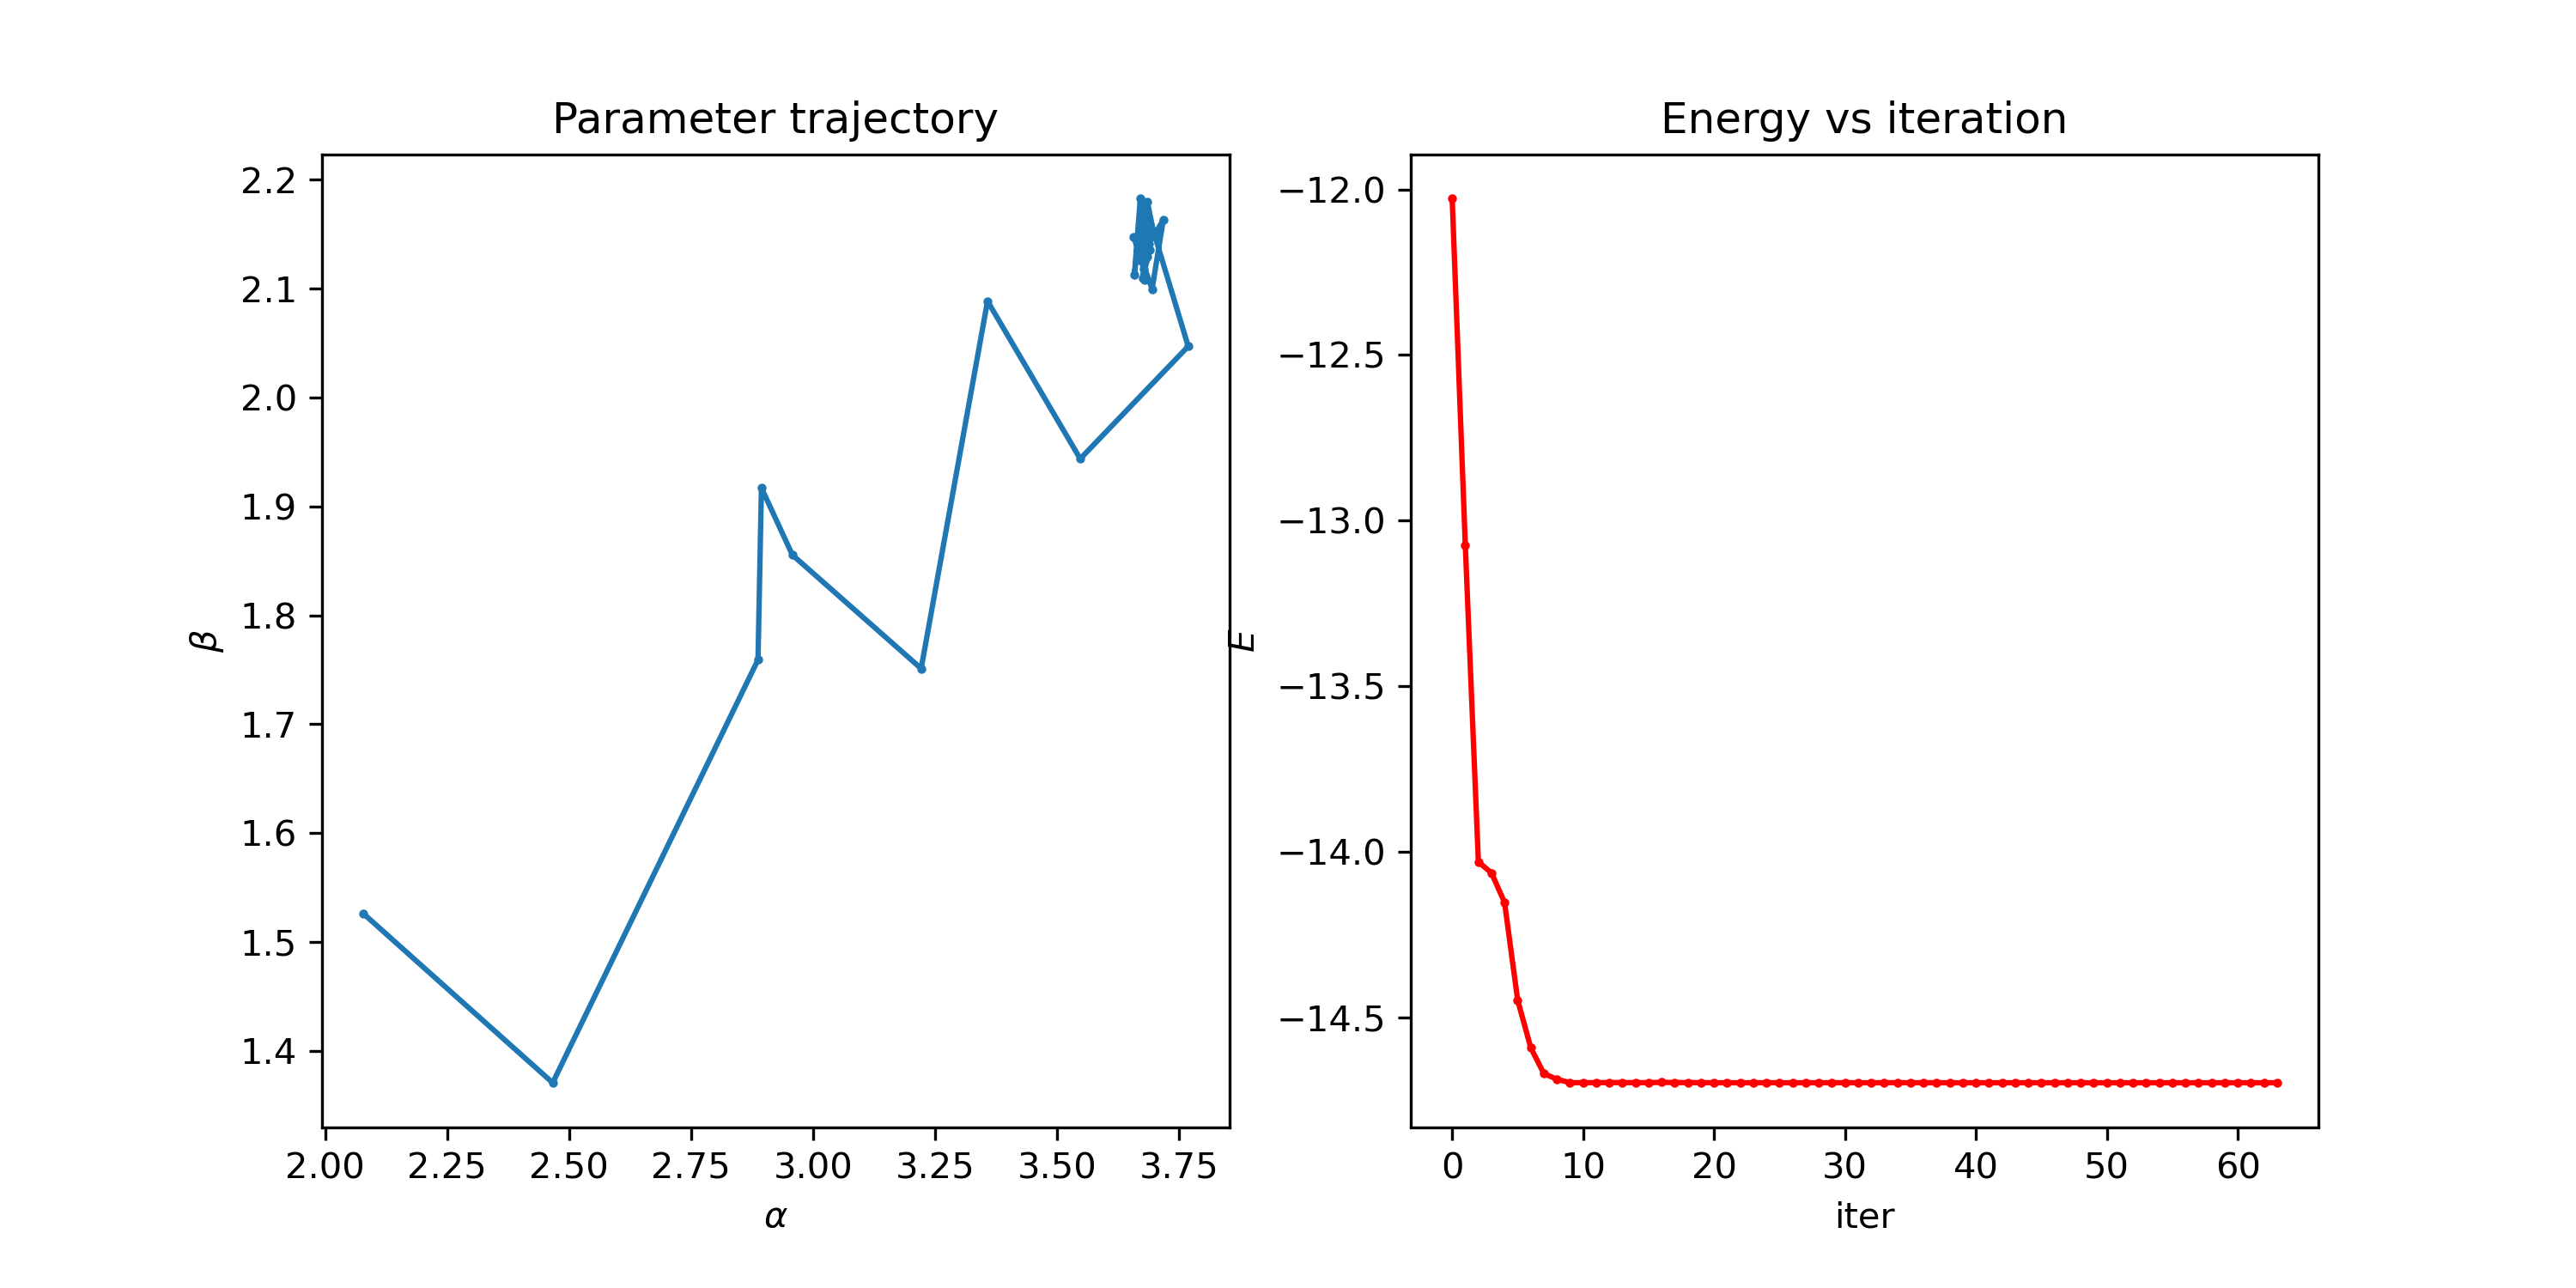
\includegraphics[width=12cm]{figs/Be_annealing.png}
    \caption{Annealing energy and parameter trajectory for Beryllium}
    \label{fig:be-scf-annealing}%
\end{figure}

Compared again with analytical result \cite{Be-perturbation} based on perturbation method. It shows both the parameters and energy agree perfectly with analytical results ($\alpha_{1s}=3.681$, $\alpha_{2s}=2.140$, $E_g=-14.698$). 

\begin{figure}[hbt!]
    \centering
    \includegraphics[width=12cm]{figs/Effective_atomic_number.png}
    \caption{Effective atomic number}
    \label{fig:effective-atmoic-number}%
\end{figure}

Since we choose the STO orbitals which are the wavefunctions for hydrogen-like atom. Parameter $\alpha$ has a physical meaning of effective charge number that tells us information about electron shielding effect. So our result shows that the effective charge number for 1s electrons is 3.68 and for 2s electrons is 2.13. This agrees with result for screening constants \cite{screening-constants} which is $Z_{1s}=3.6848$ and $Z_{2s}=1.9120$. Refer to figure \ref{fig:effective-atmoic-number}. 

Another thing worth mentioning here is that SCF is quite efficient. It took 0.24 seconds on my machine to finish 200 loops of simulated annealing. Not to mention from the figure \ref{fig:effective-atmoic-number} we can tell 200 loops are more than enough to approximate the correct answer. In this next subsection, we will see, however, VMC is not as efficient as SCF in producing result. 

\subsection{VMC--Helium}
\subsubsection*{Helium without correlation term}
Without considering correlation. VMC is expected to converge to the same energy as SCF. We iterate over $alpha$ from 1 to 2 with 0.1 as interval. Data stored in file $data/vmc/He.dat$, as is shown by figure \ref{fig:vmc-he}. Same as SCF, energy is minimized to be $-2.84$ around $\alpha = 1.7$. 
\begin{figure}
    \centering
    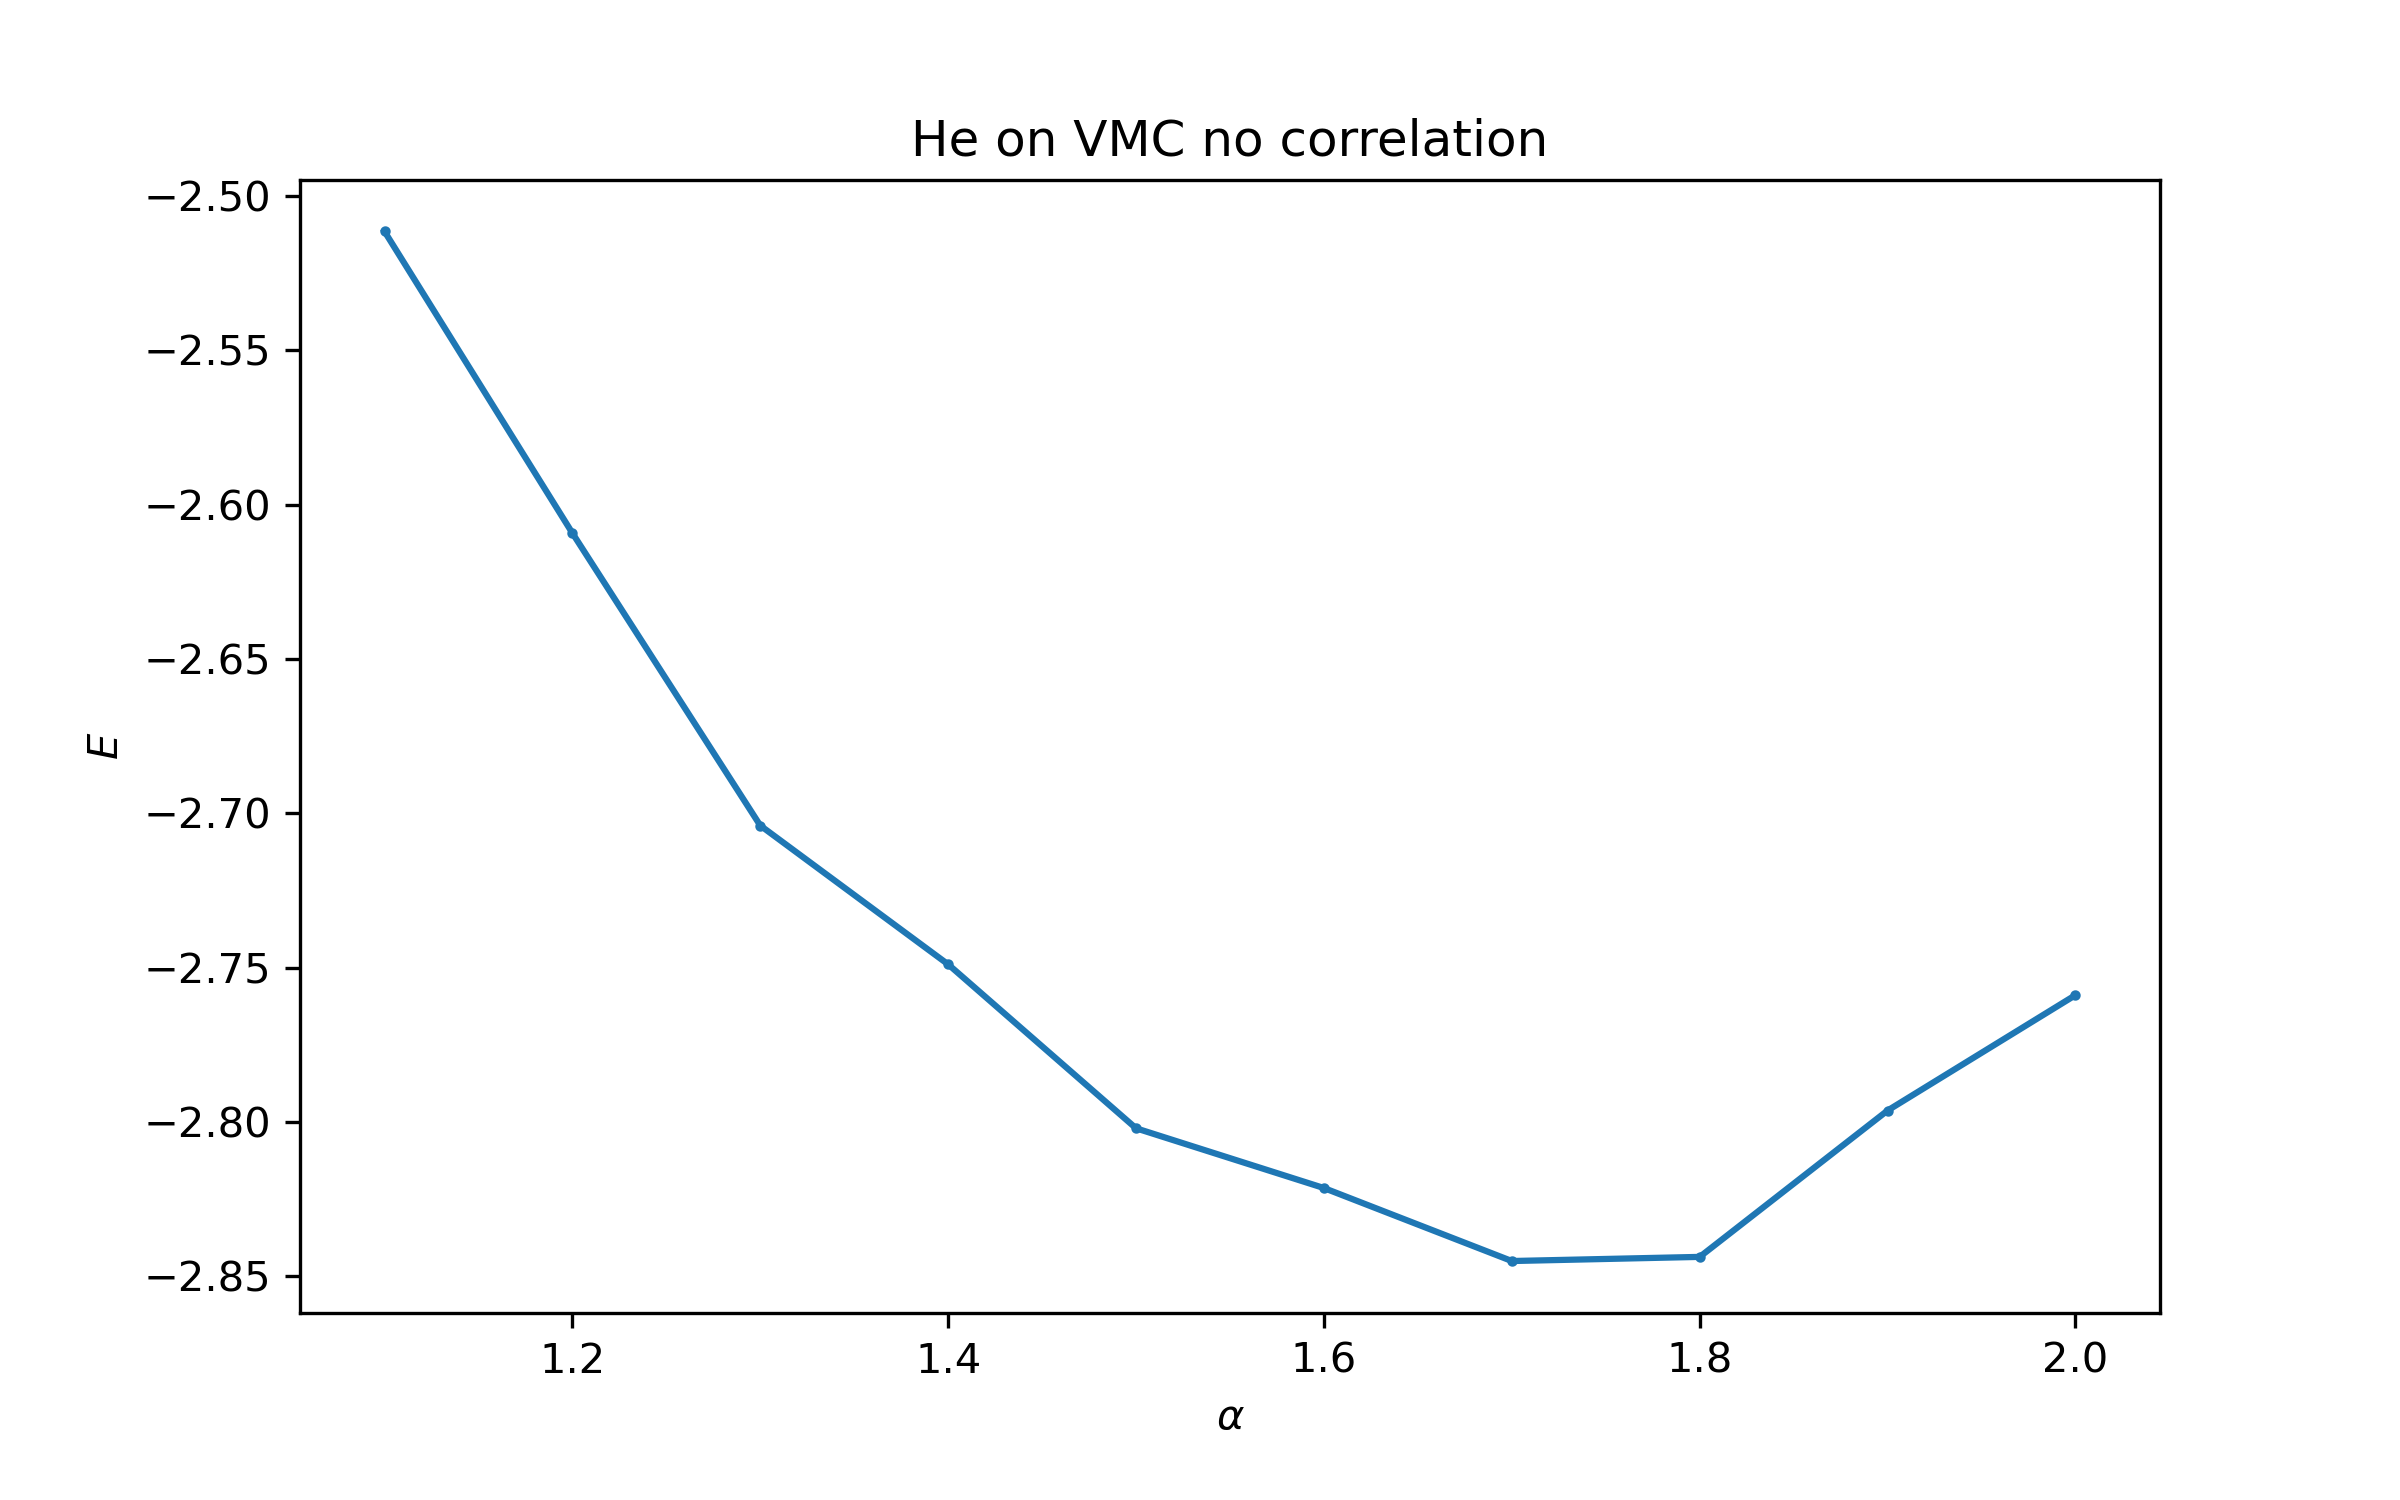
\includegraphics[width=12cm]{figs/He_without_beta.png}
    \caption{VMC for helium}
    \label{fig:vmc-he}%
\end{figure}
\subsubsection*{Helium with correlation term}
When correlation term in equation \ref{eq:atomic-wavefunction} is considered, one would expect energy would be even lower than the case without correlation. To speed up the algorithm, I vectorized the VMC algorithm by numpy.vectorize() and parallelized it by assigning 4 workers using multiprocessing.Pool(). That being said, it still took over 4 mins to finish 11 * 11 * 100000 monte carlo cycles. 

Figure \ref{fig:vmc-he-with-correlation} shows the parameter domain where energy is closed to minima, in which (a) has a 6 * 6 resolution and (b) has a 11 * 11 resolution. When $\alpha=1.8$ $\beta=1.5$, energy is minimized to be around $-2.90$, which agrees very well with the value $-2.9034$from atomic database \cite{database-he}. 

\begin{figure}
    \centering
    \subfloat[\centering 6 * 6 sample points]{{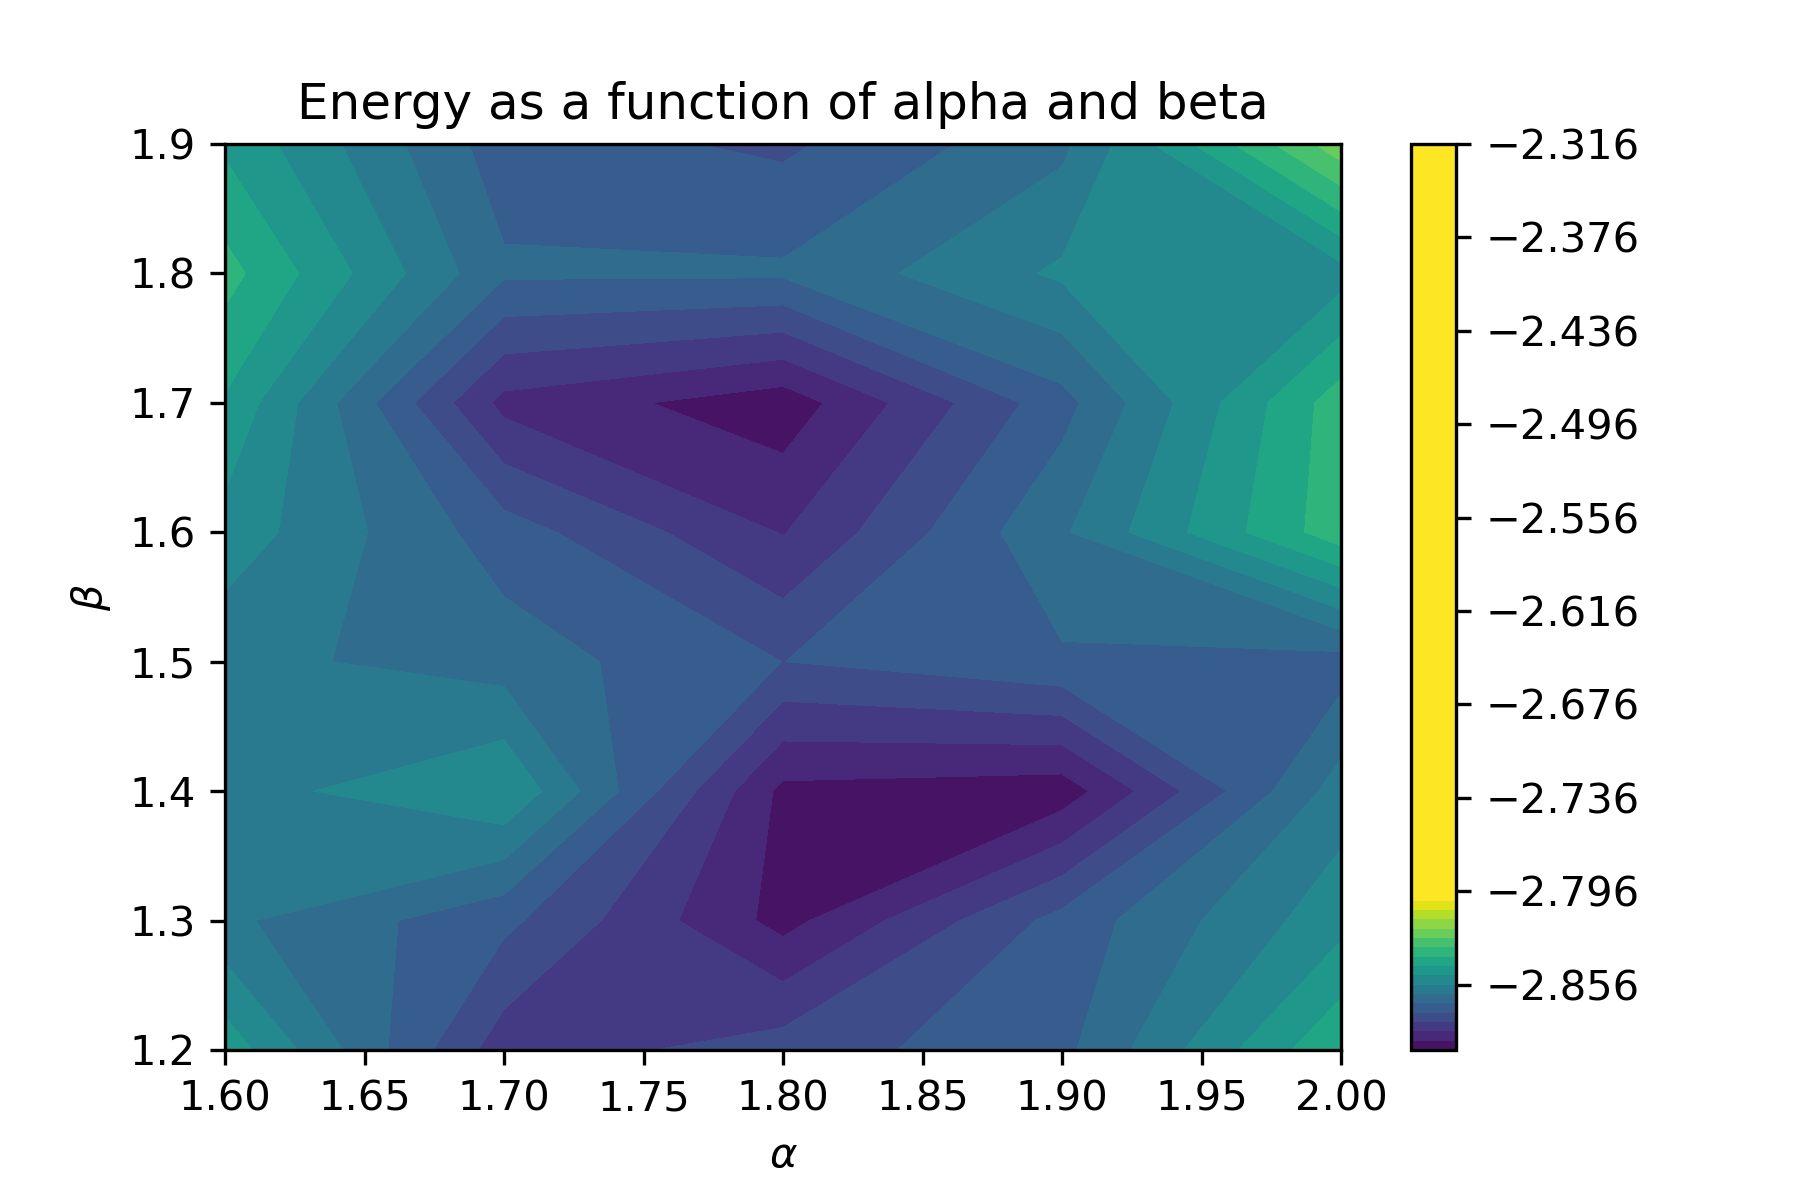
\includegraphics[width=6cm]{figs/He_with_beta.png} }}%
    \qquad
    \subfloat[\centering 11 * 11 sample points]{{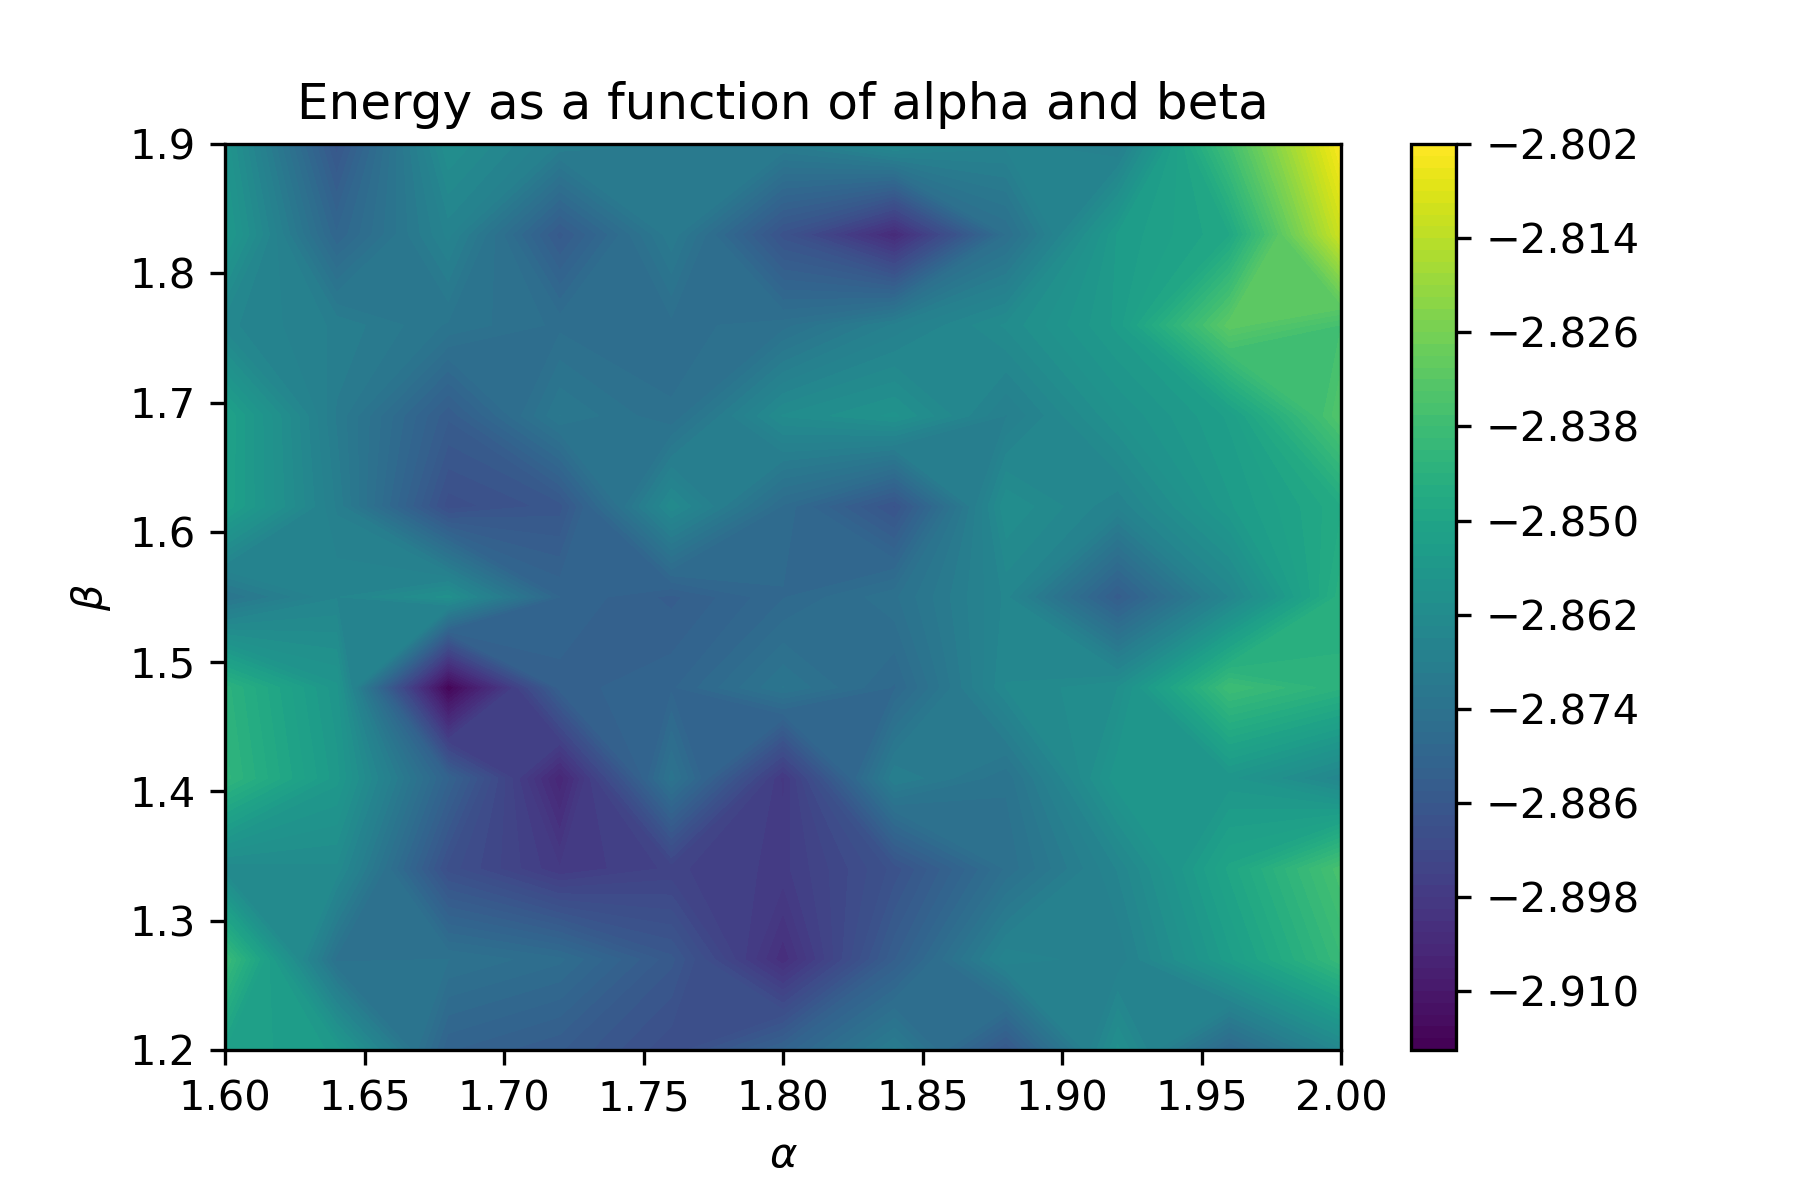
\includegraphics[width=6cm]{figs/He_with_beta_hr.png} }}%
    \caption{VMC for Helium}%
    \label{fig:vmc-he-with-correlation}%
\end{figure}


\section{Conclusion}
The SCF (Self-Consistent Field) method and the VMC (Variational Monte Carlo) method are two different approaches for calculating the ground state of a quantum many-body system.

The SCF method is a type of iterative method that starts with an initial guess for the wave function of the system, and then uses that wave function to calculate the electronic density of the system. This density is then used to construct a new wave function, which is used to calculate a new density, and so on. The process is repeated until the wave function and density converge to a self-consistent solution.

The VMC method, on the other hand, uses a variational approach to approximate the ground state wave function of the system. In this method, a trial wave function is chosen and its parameters are adjusted to minimize the energy of the system. The result is an approximate wave function that provides a good description of the ground state of the system.

In this article, we reviewed the basic concepts in SCF and VMC methods. We also implemented the SCF method for the helium and beryllium atoms and the VMC method for the helium atom with correlation term. The results show that both methods produce pretty accurate ground state energy compared with analytical and experimental data \cite{analytical_variatonal_He} \cite{Be-perturbation} \cite{database-he}. The results also show that the SCF method is more efficient than the VMC method in calculating the ground state of a quantum many-body system. But it does not incorporate the correlation term, which could be important for some types of quantum systems. It naturally follows that in order to achieve the best efficiency and accuracy, we could first solve the optimal set of $\alpha$ by using SCF method and then plug them in the VMC method, varying $\beta$ only to find the best set of $\beta$ for correlation terms. As a result, future articles could aim for combining the SCF and VMC methods in order to achieve the best trade-off of efficiency and accuracy.

\printbibliography % see references.bib for bibliography management
\end{document}